\documentclass{vs-thesis}
\setdefaultlanguage{english} % english or german 

% This package is only used in the demo and should be removed for the actual thesis.
\usepackage{blindtext}

% todo notes. (hint: remove for final version)
\usepackage[backgroundcolor=white,linecolor=red,bordercolor=red,textsize=footnotesize]{todonotes}

% Loads bibliography for citations.
\addbibresource{bibliography.bib}

% Define necessary metadata here
\title{A Truly Magnificent Demo of the VS-Thesis Template with Respect to Ridiculously Long Titles}
\thesistype{Master Thesis}
\titlegraphic{titleimage.jpg}
\submissiondate{\today}

\author{Carol Denvers}
\studentnumber{123456}
% insert specific number given by your supervisor
\internalid{VS-TODO-XYZ}
\place{Ulm}

\examiners{
    Prof.\@~Dr.-Ing.\@~Jane Doe\\
    Prof.\@~Dr.\,rer.\,nat.\@~Bruce Banner
}
\supervisors{M.Sc.\@~Arthur Dent}

\institution{
    Institute of Distributed Systems\\
    Faculty of Engineering, Computer Science and Psychology\\
    Ulm University}

\license{\ccby}

\begin{document}
    \frontmatter
    \maketitle
    \abstract{% http://www.easterbrook.ca/steve/2010/01/how-to-write-a-scientific-abstract-in-six-easy-steps/ 
The first sentence of an abstract should clearly introduce the topic of the paper so that readers can relate it to other work they are familiar with.
However, an analysis of abstracts across a range of fields show that few follow this advice, nor do they take the opportunity to summarize previous work in their second sentence.
A central issue is the lack of structure in standard advice on abstract writing, so most authors don’t realize the third sentence should point out the deficiencies of this existing research.
To solve this problem, we describe a technique that structures the entire abstract around a set of six sentences, each of which has a specific role, so that by the end of the first four sentences you have introduced the idea fully.
This structure then allows you to use the fifth sentence to elaborate a little on the research, explain how it works, and talk about the various ways that you have applied it, for example to teach generations of new graduate students how to write clearly.
This technique is helpful because it clarifies your thinking and leads to a final sentence that summarizes why your research matters.
}
    \tableofcontents

    \mainmatter
    \chapter{A multitude of tests}

\epigraph{Science is what we understand well enough to explain to a computer. Art is everything else we do.}{Donald E. Knuth}

\blindtext

\begin{figure}
    \small
    \centering
    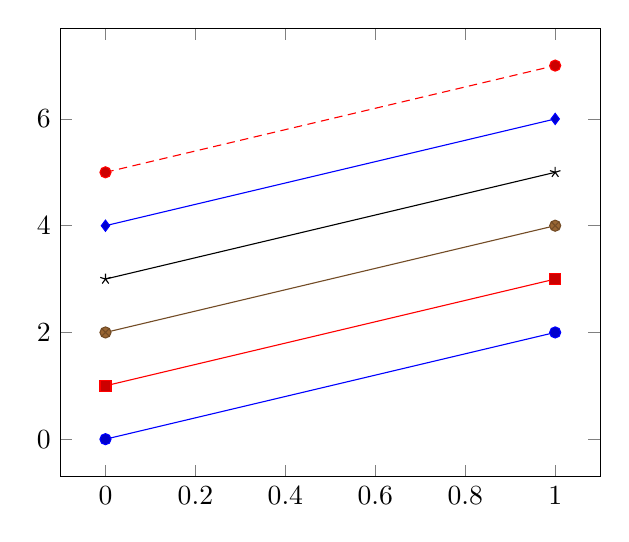
\begin{tikzpicture}
       \begin{axis}
          \addplot coordinates{(0,0) (1,2)};
          \addplot coordinates{(0,1) (1,3)};
          \addplot coordinates{(0,2) (1,4)};
          \addplot coordinates{(0,3) (1,5)};
          \addplot coordinates{(0,4) (1,6)};
          \addplot coordinates{(0,5) (1,7)};
       \end{axis}
    \end{tikzpicture}
    \caption{Just a fancy test for auto-coloring of graphs}
\end{figure}

\section{Some math}

\marginnote{This formula is also known as \emph{Pythagorean Theorem}, albeit it is usually written with the variables $a$, $b$, and $c$.}
Here follows some tests for typesetting math. Note how we use the \texttt{\\marginnote} command to add some pretty notes which appear in the margin. This is quite nice, as it allows a more narrow width of the text body without the page looking too sparse\footnote{This is a footnote}. Here comes our first equation
\begin{align}
  z^2 &= x^2 + y^2 \\
  z &= \sqrt{x^2 + y^2} \,.
\end{align}

\pagebreak
\marginnote{Did you know? The discrete fourier transformation shown in equation \cref{eqn:dft} is the backbone of the modern information-society.}
And here comes some more math, this time a discrete Fourier transformation (DFT)  which is a little bit more sophisticated than the last example\footnote{More is always better!}:
\begin{align}
	f_m =  \sum_{k=0}^{2n-1} x_k \, e^{-\frac{2\pi i}{2n} mk } \label{eqn:dft}
\qquad
m = 0,\dotsc,2n-1 \,.
\end{align}
For words of science, see~\cite{botsch2010polygon}. Unfortunately, that book has nothing about wolves.

\begin{figure}
	\small
	\centering
	\begin{tikzpicture}
		\begin{axis}[
			axis lines=left,
			scaled ticks=false,
			xticklabel style={
				rotate=90,
				anchor=east,
				/pgf/number format/precision=3,
				/pgf/number format/fixed,
				/pgf/number format/fixed zerofill,
			},
		]
		% density of Normal distribution:
		\newcommand\MU{0}
		\newcommand\SIGMA{0.1}
		\addplot+[mark=none,domain=-3*\SIGMA:3*\SIGMA,samples=201]
		{exp(-(x-\MU)^2 / 2 / \SIGMA^2)
			/ (\SIGMA * sqrt(2*pi))};
		\end{axis}
	\end{tikzpicture}
	\caption{Gaussian distribution. This plot shows a guassian distribution with mean $\mu = 0$ and standard deviation $\sigma = 0.1$. As clearly visible, the value of the distribution never reaches zero.}
	\label{fig:gaussian_distr}
\end{figure}

\section{Even more tests}
\marginnote{Blood-red were his spurs i' the golden noon; wine-red was his velvet coat, when they shot him down on the highway, down like a dog on the highway, and he lay in his blood on the highway, with the bunch of lace at his throat.}
\blindtext
\todo{write thesis}

\subsection{A test of three parts}
\blindtext

\subsection{And a second subsection}
\Blindtext

    \chapter{Another test chapter}

\begin{algorithm}
	\small
	\begin{shaded}
		\begin{algorithmic}[1]
			\newcommand*{\To}{\textbf{to}\xspace}
			\newcommand*{\Init}{\State\textbf{init}\xspace}
			\newcommand*{\B}{\mathcal{B}}
			\Init \(M \gets 0 \in \B^{N \times r}\) \Comment{Result matrix}
			\For{ \(i \gets 1\) \To N}
				\For{ \(j \gets r - r_1 + 1\) \To \(r\)}
					\State \(\ell \gets \) \Call{RandomSelect}{$\{1, \ldots, j - 1\}$} \Comment{Uniformly select set entry}
					\If{\({M}[i,\ell] = 1\)}
						\State \({M}[i,j] \gets 1\)
					\Else
						\State \({M}[i,\ell] \gets 1\)
					\EndIf
				\EndFor
			\EndFor
		\end{algorithmic}
	\end{shaded}
	\caption[Uncorrelated random data generation]{Algorithm for the generation of a block $M$ of $N$ uncorrelated random vectors of length $r$, containing exactly $r_1$ ones.}
	\label{alg:binam_random_data}
\end{algorithm}

\epigraph{To test is to live. To believe is to die.}{Anonymous Heretic}
\marginnote{Yes, this is just a test. If you read this, you are most likely doomed.}
\blindtext

\begin{figure}
    \centering
    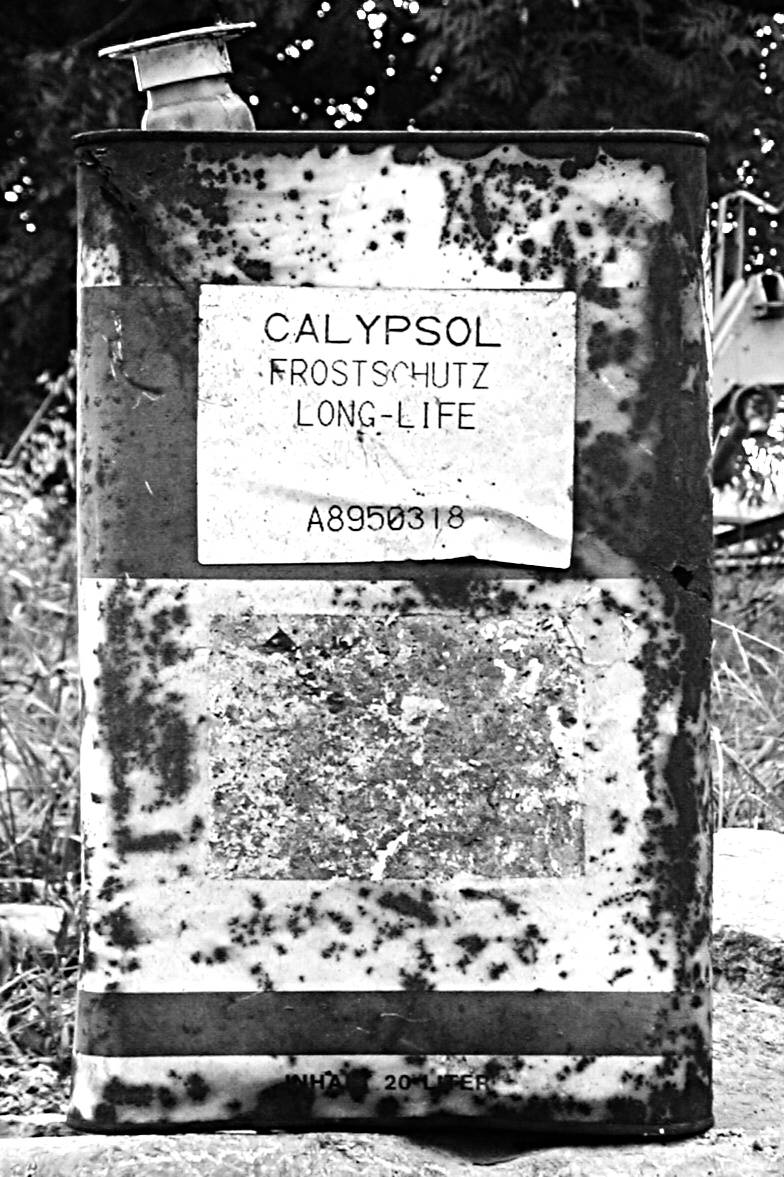
\includegraphics[width=8cm]{demo.png}
    \caption{Truly a fine canister, comparable only to mjollnir.}
    \label{fig:canister}
\end{figure}

\Blindtext\Blindtext

A picture says more than a thousand words (see \cref{fig:canister}).

\section{The Throat of the World}

\marginnote{Margin notes help to add structure to long runs of text}
\blindtext

\blindlistlist[2]{itemize}

\section{The Silence Has Been Broken}

\marginnote{Test test test}\blindtext

\blindlistlist[2]{enumerate}

\section{Discerning the Transmundane}

\marginnote{You can even add small formulas, like this one:
\begin{align*}
\sum_{i=1}^{n} i &= n \cdot \frac{n + 1}2
\end{align*}}
\blindtext

\subsection{Composure, Speed, and Precision}

\marginnote{Or this one:
\begin{align*}
E &= mc^2
\end{align*}}
\blindtext

\section{Implementation}

\blindtext

\begin{lstlisting}[caption={Very sophisticated code example.},label=lst:example]
function fizzbuzz(upperBound) {
    for (let i = 1; i < upperBound; i++) {
        if (i % 15 == 0) {
            console.log("FizzBuzz");
        } else if (i % 3 == 0) {
            console.log("Fizz");
        } else if (i % 5 == 0) {
            console.log("Buzz");
        } else {
            console.log(i);
        }
    }
}
\end{lstlisting}

    \chapter{Colors}

\blindtext

\begin{figure}[h]
    \centering
    \begin{tikzpicture}
        \foreach[count=\i] \colour in {uulm-med,uulm-mawi,uulm-nawi,uulm-in,uulm-akzent,uulm} {
            \pgfmathtruncatemacro\j{\i-1}
            \pgfmathparse{\i-0.5}
            \let\textpos\pgfmathresult
                \node[text width=2.5cm, align=right] at (-2,.5*\textpos) {\colour};
            \foreach \x in {0,1,...,9} {
                \pgfmathtruncatemacro\y{\x+1}
                \pgfmathparse{100-\x*10}
                \let\saturation\pgfmathresult
                    \fill[\colour!\saturation] (.5*\x,.5*\j) rectangle (.5*\y,.5*\i);
            }
        }
    \end{tikzpicture}
    \caption{The Ulm University Colour Palette\cite{cd}}
\end{figure}

\blindtext

\begin{table}
    \centering
    \renewcommand{\arraystretch}{1.3}
    \scriptsize
    \begin{tabular}{lp{3.2cm}lll}
        \textbf{Color Macro} & \textbf{Association}  & \textbf{CMYK} & \textbf{sRGB} & \textbf{Hex} \\\midrule 
        uulm & Ulm University  & C30-mo-yo-k35 & 125-154-170 & \#7D9AAA \\
        uulm-akzent & Emphasis Colour  & C0-mo-y28-k38 & 169-162-141 & \#A9A280\\
        uulm-in & Engineering, Computer\newline Science, and Psychology & C0-m100-y63-k29 & 163-38-56 & \#A32638 \\
        uulm-nawi & Natural Sciences & C0-m66-y100-k7 & 189-96-5 & \#BD6005 \\
        uulm-mawi & Mathematics and\newline Economics & C59-mo-y100-k7 & 86-170-28 & \#56AA1C \\
        uulm-med & Medicine & C100-m56-yo-k23 & 38-84-124 & \#26247C\\
    \end{tabular}
    \caption{Color Definition of the Ulm University Colors~\cite{cd}}
\end{table}


    \backmatter
    \printbibliography[heading=bibintoc]
\end{document}
